\chapter{Расчёт параметров}

\section{Расчёт относительного уменьшения возбуждения на краю антенны}

Чтобы обеспечить заданный уровень боковых лепестков, воспользуемся распределением возбуждения <<косинус на пьедестале>>
\[
    I(z) = 1 + \Delta \cos \frac{2 \pi z}{L}\text{, }|z| \leq \frac{L}{2},
\]
при котором уровень боковых лепестков равен
\[
    t \approx -(13 + 13 \Delta + 22 \Delta^2),
\]
откуда $\Delta \approx 0.127$.

\section{Расчёт межэлементного расстояния}

Достаточно малый угол сканирования позволяет применить <<мягкую>> формулу, представляющую собой следствие теоремы перемножения в теории антенн.
В соответствии с этой формулой, полная \gls{directivity} антенной решётки является произведением \gls{directivity} одного элемента на множитель направленности решётки.
следствием этого является подавление побочного максимума излучения, если один из элементов имеет незначительное излучение.

\[
    d \leq \frac{\lambda}{\sin\Theta_\text{д} + \sin\Theta_\text{ск}},
\]
где $\Theta_{д}$ --- направление дифракционного максимума.
Определим его, воспользовавшись формулой для аппроксимации \gls{directivity} элемента:
\[
    f^2(\Theta) = \cos^{2 \alpha} \Theta = \frac{1}{2},
\]
откуда
\[
    \alpha = \frac{1}{2} \frac{\lg{0.5}}{\lg{\cos \Theta_\text{ск}}}.
\]

Значение $\Theta_\text{д}$ определяется из соображение, что при отклонении основного лепестка на предельное значение $\Theta_\text{д}$ дифракционный максимум подавляется \gls{directivity} элемента на $3~\text{дБ}$ до допустимого \gls{sidelobelevel} $t$:
\[
    f^2(\Theta_\text{д}) = \cos^{2 \alpha} \Theta_\text{д} \leq t,
\]
откуда находим предельное значение $\Theta_\text{д} = \arccos \sqrt[2 \alpha]{t}$.

Воспользуемся полученными формулами для расчёта по каждой из осей:
\begin{enumerate}
    \item
        Ось $x$: $\alpha_x \approx 9.997$, $\Theta_{\text{д} x} \approx 32.72^\circ$, $d_x \approx 6.26~\text{см}$;
    \item
        Ось $y$: $\alpha_y \approx 2.409$, $\Theta_{\text{д} y} \approx 60.77^\circ$, $d_y \approx 3.64~\text{см}$.
\end{enumerate}

\section{Расчёт количества элементов}

Воспользуемся формулой $\frac{(1 + 0.636 \Delta^2) \cdot 51^\circ \cdot \lambda}{\Theta_{0.5} \cdot d}$ для вычисления количества элементов на каждой из сторон решётки:
\begin{enumerate}
    \item
        Ось $x$: $N_x = 14$;
    \item
        Ось $y$: $N_y = 12$.
\end{enumerate}
Общее число элементов решётки в тогда равно $N = N_x \cdot N_y = 168$.

\section{Расчёт энергетического потенциала АФАР и выбор схемы разводки}

Заложим следующие потери в схеме разводки:
\begin{itemize}
    \item Потери во входном фильтре и соединительных кабелях: $1~\text{дБ}$;
    \item Потери в фазовращателе и юстировочном фазовращателе: $3~\text{дБ}$;
    \item Омические потери в одном делителе на 2: $0.5~\text{дБ}$;
    \item Потери в соединительных кабелях: $1~\text{дБ/м}$;
    \item Потери в соединительном кабеле между АФАР и приёмником: $0.5~\text{дБ}$.
\end{itemize}

Рассмотрим одноэтажную схему разводки (Рис.~\ref{fig:structure-schematic}).
Используем сумматор с 256 входами, где неиспользуемые входы включены на согласованную нагрузку по схеме ниже.
\begin{figure}[H]
    \centering
    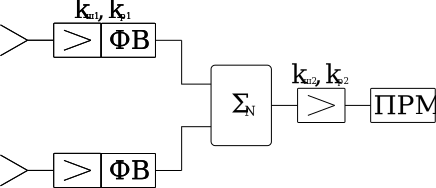
\includegraphics[width=0.9\textwidth]{structure-schematic}
    \caption{Структурная схема приёмной АФАР}%
    \label{fig:structure-schematic}
\end{figure}

Схема прохождения сигнала по одному канала представлена на рис.~\ref{fig:structure-schematic-channel}.
\begin{figure}[H]
    \centering
    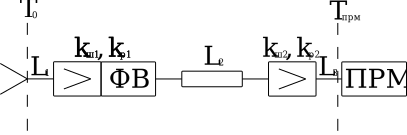
\includegraphics[width=0.9\textwidth]{structure-schematic-channel}
    \caption{Структурная схема канала приёмной АФАР}%
    \label{fig:structure-schematic-channel}
\end{figure}
На данном рисунке используются следующие обозначения:
\begin{itemize}
    \item $K_p = 17~\text{дБ} \approx 50$ --- коэффициент усиления каждого МШУ;
    \item $K_\text{ш} = 3.5~\text{дБ} \approx 2.2$ --- коэффициент шума каждого МШУ;
    \item $L_1 = 0.8~\text{дБ} \approx 1.2$ --- потери в соединительном кабеле между излучателем и МШУ, а также потери во входном фильтре МШУ;
    \item $L_2 = L_\text{ФВ} + L_\text{фид} + L_{1 \sum} \cdot N_\text{э} = 1~\text{дБ} + 3~\text{дБ} + 8 \cdot 0.5~\text{дБ} = 8~\text{дБ} \approx 6.3$ --- суммарные потери в фазовращателе, юстировочном фазовращателе, сумматоре и соединительных кабелях для восьмиуровнего делителя;
    \item $L_3 = 0.5~\text{дБ} \approx 1.1$ --- потери в соединительном кабеле между вторым МШУ и приёмником, которые в дальнейших расчётах опускаются в связи с незначительным вкладом.
\end{itemize}

Имеем
\[
    K_{\text{ш}\Sigma}
    = K_\text{ш} L_1 + \frac{(L_2 - 1) L_1}{K_p} + \frac{(K_\text{ш} - 1) L_2 L_1}{K_p}
    = 2.2 \cdot 1.2 + \frac{(6.3 - 1) \cdot 1.2}{50} + \frac{(2.2 - 1) \cdot 6.3 \cdot 1.2}{50}
    \approx 2.95
\]
Второе и третье слагаемые суммы коэффициентов шума превышает первое более чем на 10~\%.
Для уменьшения влияния потерь при суммировании целесообразно применить активную разводку с двухканальной схемой.
Разобьём всю решётку на 32 подрешётки по 8 элементов (Рис.~\ref{fig:subarrays}) исходя из соображения, что количество уровней сумматора между первым МШУ и вторым должно быть как можно меньшим, т.к. соответствующее слагаемое вносит большой вклад в суммарный коэффициент шума, но подрешёток не должно быть слишком много в силу того, что это увеличивает стоимость итогового изделия.
\begin{figure}[H]
    \centering
    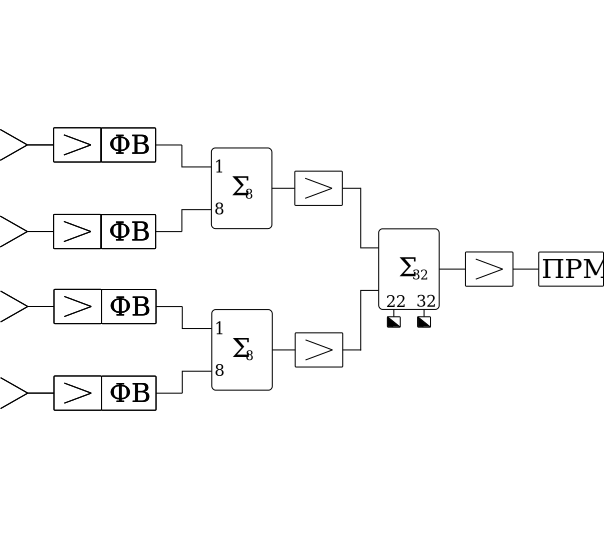
\includegraphics[width=0.9\textwidth]{subarrays}
    \caption{Разбиение на подрешётки}%
    \label{fig:subarrays}
\end{figure}
Неиспользованные входы сумматоров включены на согласованные нагрузки.
Так как не используются одинадцать входов (Рис.~\ref{fig:subarrays}), то целесообразно поставить нагрузки не на первом уровне, а на уровнях 1, 2 и 4, что позволит сократить количество необходимых согласованных нагрузок с одинадцати до трёх.

\section{Энергетический потенциал}

Рассчитаем энергетический потенциал АФАР.
\[
    \Pi_\text{прм}
    = \frac{S_\text{эфф}}{T_\text{эфф}},
\]
где $S_\text{эфф}$ --- эффективная площадь АФАР, $T_\text{эфф}$ --- приведённая к раскрыву решётки шумовая температура АФАР.
Найдём их.
\[
    S_\text{эфф}
    = A \cdot S_t \cdot \sigma
    = 0.5 \cdot (87.64 \cdot 43.68) \cdot 0.7
    \approx 1340~\text{см}^2,
\]
\[
    T_\text{эфф}
    = T_0 \cdot (K_{\text{ш}\Sigma} - 1)
    = 290 \cdot (2.95 - 1)
    \approx 566~\text{К},
\]
откуда окончательно
\[
    \Pi_\text{прм}
    = \frac{1340}{566},
    \approx 2.4~\text{см}^2\text{/К}.
\]

\section{Точность выставки луча}

Ошибка наведения луча антенной решётки может быть найдена по формуле
\[
    \delta \Theta
    = \frac{9 \cdot \Delta \Theta_{0.5}}{N \cdot 2^p}.
\]
Подставив значения, получим $\delta \Theta_x = 0.24^\circ$ и $\delta \Theta_y = 0.56^\circ$ по осям $x$ и $y$ соответственно.

\section{Выбор типа излучателя}
Угол сканирования достаточно мал и отличается по осям $x$ и $y$, поэтому в качестве излучателя следует выбрать рупорную антенну.
Параметры выбранной рупорной антенны будут следующими:
\begin{itemize}
    \item $a \times b = 35 \times 15~\text{мм}$ --- основание рупора, размеры которого равны размеру ГОСТированного волновода для данной частоты;
    \item $d_1 \times d_2 = 62.6 \times 36.4~\text{мм}$ --- размеры раскрыва рупора.
    \item $R = \cfrac{1}{3} \cdot \cfrac{d_1^2}{5} = 26.1~\text{мм}$ --- длина рупора вдоль оси $z$;
\end{itemize}
